
\documentclass[border=10pt, 12pt]{standalone}
\usepackage[svgnames]{xcolor}
\usepackage{amsmath}
\usepackage{pgfplots}
\pgfplotsset{compat=newest}
\usepackage[sfdefault]{FiraSans}
\usepackage{FiraMono}
\renewcommand*\familydefault{\sfdefault}
\begin{document}
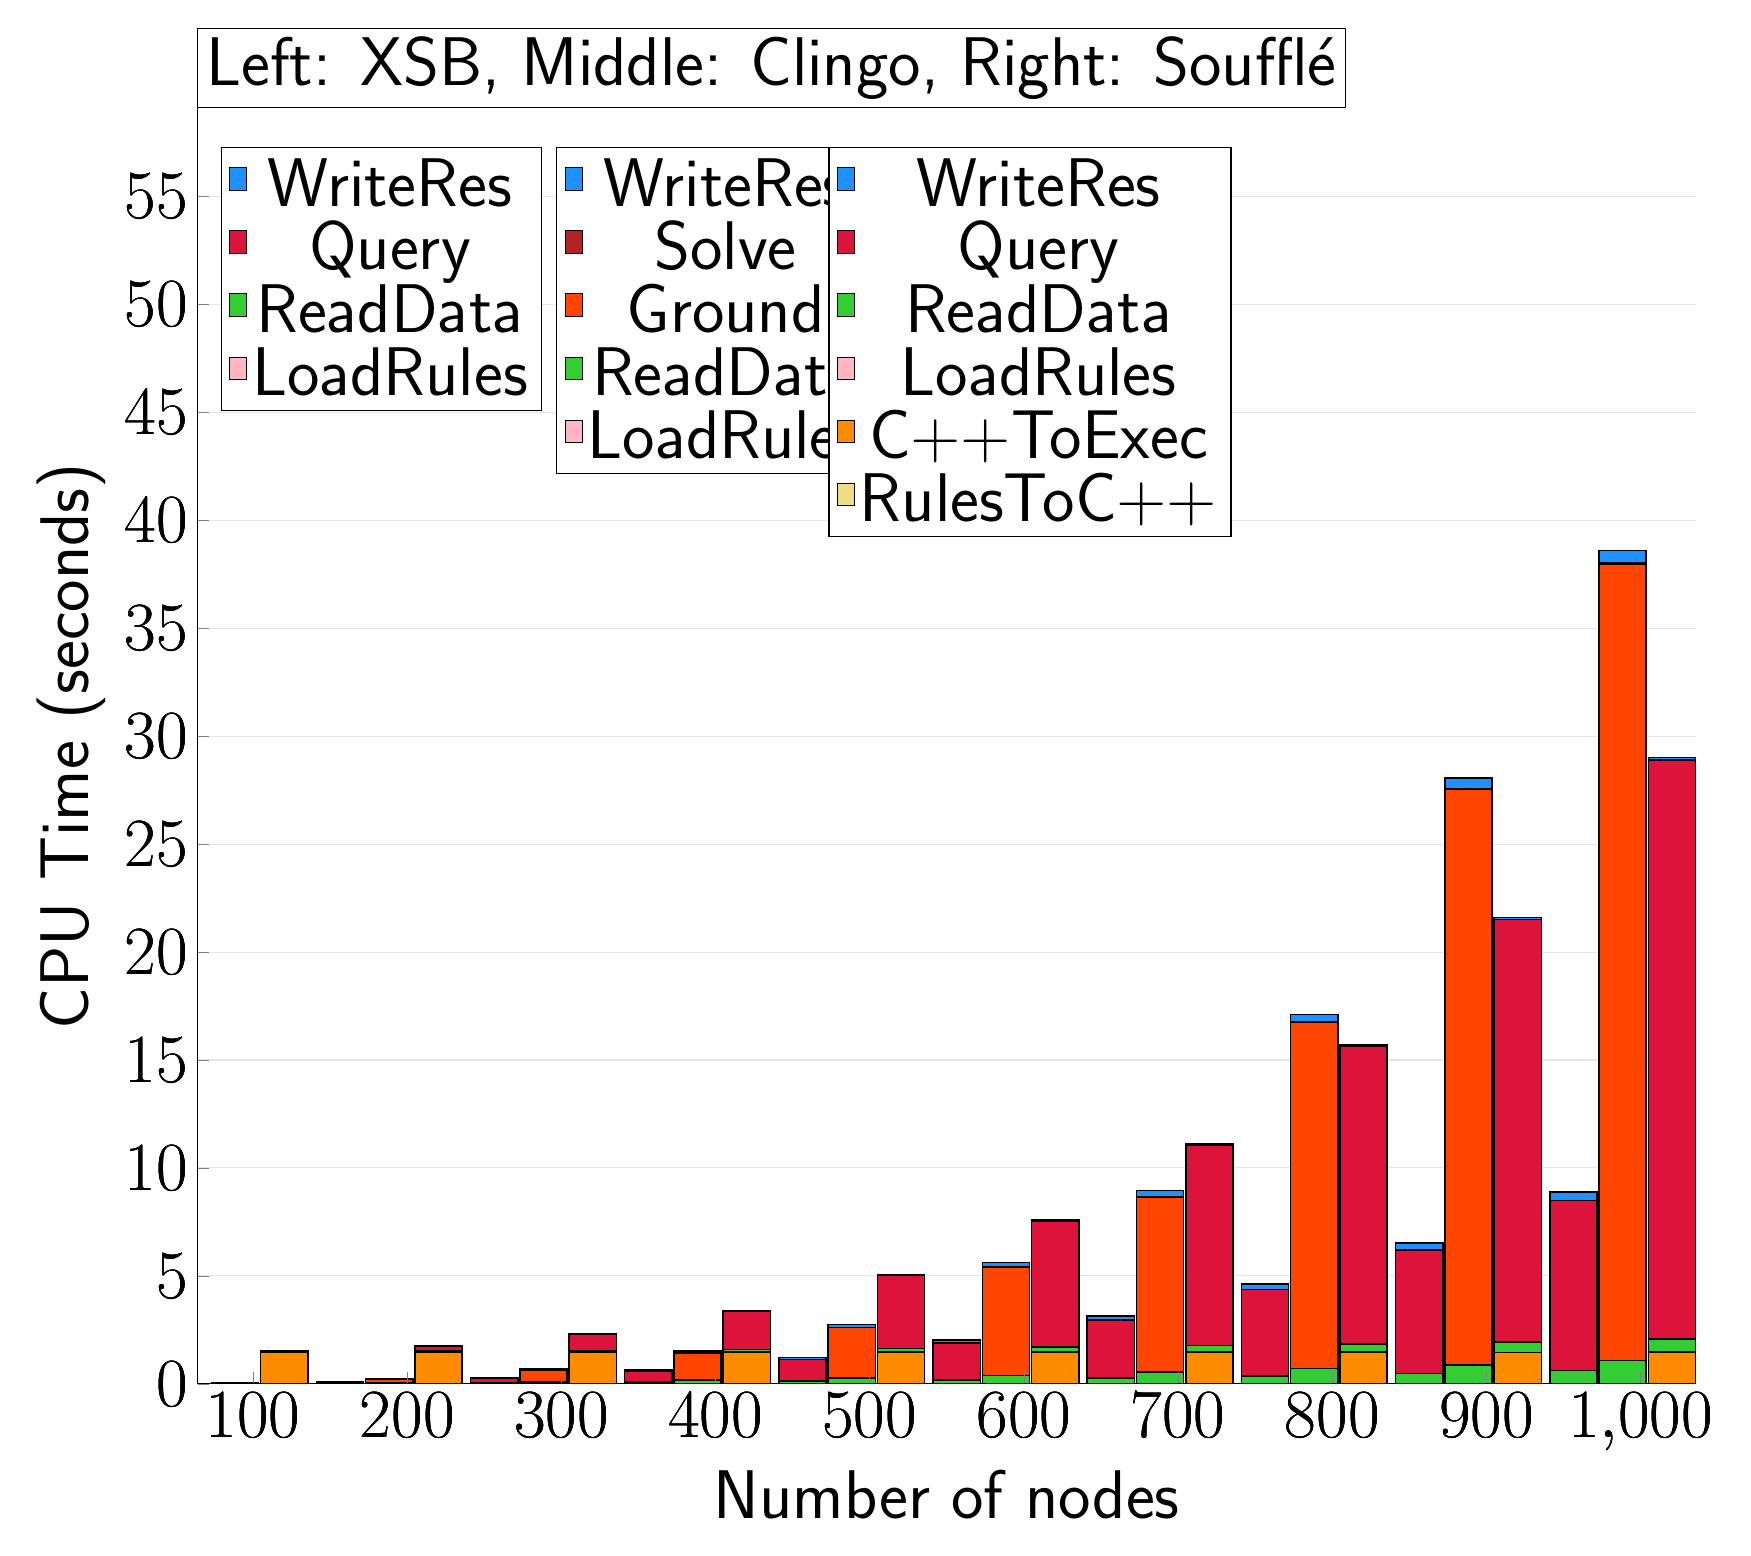
\begin{tikzpicture}
                        \begin{axis}[bar shift=-24.3pt, 
   ybar stacked,
   width=1.7\textwidth,
   bar width=0.6cm,
   ymajorgrids, tick align=inside,
   major grid style={draw=gray!20},
   xtick=data,
   ymin=0, ymax=59.082040000000006,
   axis x line*=bottom,
   axis y line*=left,
   enlarge x limits=0.04,
   legend style={
       at={(0.23, 0.97)},
       anchor=north east,
       legend columns=1,
       font=\Huge,
   },
   ylabel={CPU Time (seconds)},
   xlabel={Number of nodes},
   label style={font=\Huge},
   tick label style={font=\Huge},
]
\addlegendimage{fill=DodgerBlue, draw=black, line width=0.2pt}
\addlegendentry{WriteRes}
\addlegendimage{fill=Crimson, draw=black, line width=0.2pt}
\addlegendentry{Query}
\addlegendimage{fill=LimeGreen, draw=black, line width=0.2pt}
\addlegendentry{ReadData}
\addlegendimage{fill=LightPink, draw=black, line width=0.2pt}
\addlegendentry{LoadRules}
\addplot +[fill=LightPink, draw=black, line width=0.55pt] coordinates {
(100, 0.0005519999999999998)
(200, 0.000553)
(300, 0.000551)
(400, 0.0005531999999999998)
(500, 0.0005528000000000002)
(600, 0.0005619999999999998)
(700, 0.0005554000000000003)
(800, 0.0005547999999999997)
(900, 0.0005510000000000004)
(1000, 0.0005592)
};
\addplot +[fill=LimeGreen, draw=black, line width=0.55pt] coordinates {
(100, 0.0040447999999999994)
(200, 0.0170934)
(300, 0.040194999999999995)
(400, 0.07461960000000001)
(500, 0.1219422)
(600, 0.1840564)
(700, 0.26083680000000004)
(800, 0.3577032)
(900, 0.46859779999999995)
(1000, 0.6110244)
};
\addplot +[fill=Crimson, draw=black, line width=0.55pt] coordinates {
(100, 0.0081346)
(200, 0.0646892)
(300, 0.2161836)
(400, 0.5093488)
(500, 1.0045911999999997)
(600, 1.7000406)
(700, 2.6842528)
(800, 4.010453)
(900, 5.7381466)
(1000, 7.883575800000001)
};
\addplot +[fill=DodgerBlue, draw=black, line width=0.55pt] coordinates {
(100, 0.0040352)
(200, 0.016613)
(300, 0.03637000000000001)
(400, 0.06663279999999998)
(500, 0.10192140000000002)
(600, 0.15044999999999997)
(700, 0.20661520000000005)
(800, 0.25999580000000017)
(900, 0.3189255999999997)
(1000, 0.3932047999999998)
};
\end{axis}

\begin{axis}[bar shift=-6.5pt, 
   ybar stacked,
   width=1.7\textwidth,
   bar width=0.6cm,
   ymajorgrids, tick align=inside,
   major grid style={draw=none},
   xtick=data,
   ymin=0, ymax=59.082040000000006,
   axis x line*=none,
   axis y line*=none,
   enlarge x limits=0.04,
   legend style={
       at={(0.454, 0.97)},
       anchor=north east,
       legend columns=1,
       font=\Huge,
   },
   label style={font=\Huge},
   tick label style={font=\Huge},
]
\addlegendimage{fill=DodgerBlue, draw=black, line width=0.2pt}
\addlegendentry{WriteRes}
\addlegendimage{fill=FireBrick, draw=black, line width=0.2pt}
\addlegendentry{Solve}
\addlegendimage{fill=OrangeRed, draw=black, line width=0.2pt}
\addlegendentry{Ground}
\addlegendimage{fill=LimeGreen, draw=black, line width=0.2pt}
\addlegendentry{ReadData}
\addlegendimage{fill=LightPink, draw=black, line width=0.2pt}
\addlegendentry{LoadRules}
\addplot +[fill=LightPink, draw=black, line width=0.55pt] coordinates {
(100, 0.0)
(200, 0.0)
(300, 0.0)
(400, 0.0)
(500, 0.0)
(600, 0.0)
(700, 0.0)
(800, 0.0)
(900, 0.0)
(1000, 0.0)
};
\addplot +[fill=LimeGreen, draw=black, line width=0.55pt] coordinates {
(100, 0.010000000000000009)
(200, 0.040000000000000036)
(300, 0.09200000000000003)
(400, 0.16999999999999998)
(500, 0.268)
(600, 0.38599999999999995)
(700, 0.5360000000000001)
(800, 0.7040000000000001)
(900, 0.874)
(1000, 1.0879999999999999)
};
\addplot +[fill=OrangeRed, draw=black, line width=0.55pt] coordinates {
(100, 0.020000000000000018)
(200, 0.15799999999999997)
(300, 0.554)
(400, 1.252)
(500, 2.332)
(600, 5.008)
(700, 8.108)
(800, 16.028000000000002)
(900, 26.682)
(1000, 36.894000000000005)
};
\addplot +[fill=FireBrick, draw=black, line width=0.55pt] coordinates {
(100, 0.0)
(200, 0.0020000000000000018)
(300, 0.0020000000000000018)
(400, 0.0040000000000000036)
(500, 0.007999999999999919)
(600, 0.010000000000000142)
(700, 0.013999999999999702)
(800, 0.021999999999999176)
(900, 0.0260000000000002)
(1000, 0.03400000000000074)
};
\addplot +[fill=DodgerBlue, draw=black, line width=0.55pt] coordinates {
(100, 0.010000000000000009)
(200, 0.018000000000000016)
(300, 0.05199999999999998)
(400, 0.09600000000000009)
(500, 0.14400000000000013)
(600, 0.20999999999999983)
(700, 0.28800000000000037)
(800, 0.35800000000000093)
(900, 0.4759999999999994)
(1000, 0.5819999999999992)
};
\end{axis}

\begin{axis}[bar shift=11.3pt, 
   ybar stacked,
   width=1.7\textwidth,
   bar width=0.6cm,
   ymajorgrids, tick align=inside,
   major grid style={draw=none},
   xtick=data,
   ymin=0, ymax=59.082040000000006,
   axis x line*=none,
   axis y line*=none,
   enlarge x limits=0.04,
   legend style={
       at={(0.69, 0.97)},
       anchor=north east,
       legend columns=1,
       font=\Huge,
   },
   label style={font=\Huge},
   tick label style={font=\Huge},
]
\addlegendimage{fill=DodgerBlue, draw=black, line width=0.2pt}
\addlegendentry{WriteRes}
\addlegendimage{fill=Crimson, draw=black, line width=0.2pt}
\addlegendentry{Query}
\addlegendimage{fill=LimeGreen, draw=black, line width=0.2pt}
\addlegendentry{ReadData}
\addlegendimage{fill=LightPink, draw=black, line width=0.2pt}
\addlegendentry{LoadRules}
\addlegendimage{fill=DarkOrange, draw=black, line width=0.2pt}
\addlegendentry{C++ToExec}
\addlegendimage{fill=LightGoldenrod, draw=black, line width=0.2pt}
\addlegendentry{RulesToC++}
\addplot +[fill=LightGoldenrod, draw=black, line width=0.55pt] coordinates {
(100, 0.004000000000000001)
(200, 0.006000000000000001)
(300, 0.004000000000000001)
(400, 0.006000000000000001)
(500, 0.0020000000000000005)
(600, 0.008000000000000002)
(700, 0.004000000000000001)
(800, 0.004000000000000001)
(900, 0.006000000000000001)
(1000, 0.0020000000000000005)
};
\addplot +[fill=DarkOrange, draw=black, line width=0.55pt] coordinates {
(100, 1.462)
(200, 1.4679999999999997)
(300, 1.462)
(400, 1.472)
(500, 1.47)
(600, 1.466)
(700, 1.464)
(800, 1.4620000000000002)
(900, 1.4540000000000002)
(1000, 1.476)
};
\addplot +[fill=LightPink, draw=black, line width=0.55pt] coordinates {
(100, 0.0001538)
(200, 0.00016099999999999998)
(300, 0.00015759999999999998)
(400, 0.00016319999999999998)
(500, 0.0001574)
(600, 0.0001258)
(700, 0.0001676)
(800, 0.000154)
(900, 0.0)
(1000, 0.0001572)
};
\addplot +[fill=LimeGreen, draw=black, line width=0.55pt] coordinates {
(100, 0.0147896)
(200, 0.041839)
(300, 0.07426840000000001)
(400, 0.11435339999999998)
(500, 0.1649852)
(600, 0.22475879999999998)
(700, 0.3053518)
(800, 0.3890866)
(900, 0.4648958)
(1000, 0.5973258)
};
\addplot +[fill=Crimson, draw=black, line width=0.55pt] coordinates {
(100, 0.0431402)
(200, 0.2293734)
(300, 0.7472768000000001)
(400, 1.752296)
(500, 3.4048660000000006)
(600, 5.849704)
(700, 9.288908000000001)
(800, 13.80174)
(900, 19.59016)
(1000, 26.823040000000002)
};
\addplot +[fill=DodgerBlue, draw=black, line width=0.55pt] coordinates {
(100, 0.0014248)
(200, 0.0044564)
(300, 0.0099576)
(400, 0.0173284)
(500, 0.026957799999999997)
(600, 0.038592)
(700, 0.0522776)
(800, 0.06780800000000001)
(900, 0.0859326)
(1000, 0.10569139999999999)
};
\end{axis}


\node[anchor=south, draw, fill=white] at (rel axis cs:0.42,1) {\Huge Left: XSB, Middle: Clingo, Right: Soufflé};
\end{tikzpicture}
\end{document}
                    